% System description paper, Sinhala MMLU Shared Task @ ICTer 2026. ACL style; compile with XeLaTeX:
%   python make_prompt_tex.py && python make_appendix_tex.py
%   latexmk -xelatex SinhalaMMLU2026_team-sinbotics_SystemReport.tex
\documentclass[11pt]{article}
\usepackage[preprint]{acl}
\usepackage{fontspec}
\setmainfont{Times New Roman}
\setmonofont{Consolas}[Scale=0.88]
\newfontfamily\sinhalafont{Nirmala UI}[Script=Sinhala]
\newfontfamily\symbolfont{Segoe UI Symbol}
\usepackage{amsmath}
\usepackage{booktabs}
\usepackage{array}
\usepackage{tabularx}
\usepackage{longtable}
\usepackage{xcolor}
\usepackage{tikz}
\usetikzlibrary{positioning}

\newcommand{\si}[1]{{\sinhalafont #1}}
\newcommand{\sinhalatext}[1]{{\sinhalafont #1}}
\newcommand{\cond}[1]{\texttt{#1}}
\definecolor{best}{RGB}{0,100,0}
\newcommand{\best}[1]{\textbf{\textcolor{best}{#1}}}
\newcommand{\ticked}{{\symbolfont ☒}}
\newcommand{\unticked}{{\symbolfont ☐}}
\newcommand{\para}[1]{\smallskip\noindent\textbf{#1}\enspace}
\renewcommand{\textvisiblespace}{\mbox{\kern.06em\vrule height.3ex\vbox{\hrule width.3em}\vrule height.3ex\kern.06em}}
\newcommand{\repo}{SinhalaMMLU-SharedTask/team-sinbotics}
\newcommand{\sinmulu}{Sinmulu\_si}
\newcolumntype{L}[1]{>{\raggedright\arraybackslash}p{#1}}
\newcolumntype{Y}{>{\raggedright\arraybackslash}X}
\urlstyle{same}
\setlength{\tabcolsep}{3.5pt}
\raggedbottom

\title{SinBotics at Sinhala MMLU 2026: LoRA-Tuned Qwen3.5-4B\\Thinking in English about Sinhala Questions}

\author{Sachintha Weththasinghe \\ SLIIT \And
  Hasitha Hirushan \\ SLIIT \And
  Hasaan Saadhiq \\ SLIIT \And
  Janith Ramanayake \\ University of Moratuwa}

\begin{document}
\maketitle

\begin{abstract}
We describe the SinBotics system for the Sinhala MMLU Shared Task at ICTer 2026. The system combines Qwen3.5-4B with a rank-16 LoRA adapter, for a total of 4.24B parameters, and the adapter was trained for one epoch on 25,799 Sinhala multiple-choice questions drawn from Global-MMLU Sinhala and \sinmulu{}, a new collection of Sri Lankan exam questions. At inference, the model reads the original Sinhala question and, acting as a Sri Lankan teacher of the subject, reasons step by step in English using Qwen's thinking mode; the most probable digit from 1 to 4 is then taken as the answer. We selected this configuration by comparing full systems on a 300-question screening set. The system ranked 11th with a \textbf{Macro Avg of 57.58\%} (Easy 54.67, Medium 52.30, Hard 65.77).
\end{abstract}

{\small\noindent\textbf{Team information.} Team SinBotics; Codabench user sachintha\_akalanka; contact: Sachintha Weththasinghe, akalankasachintha125@gmail.com. Code, inference script, predictions and adapter: \url{https://huggingface.co/SinhalaMMLU-SharedTask/team-sinbotics}.\par}

\section{Introduction}
SinhalaMMLU \citep{pramodya2025sinhalammlu} is the first multitask language-understanding benchmark for Sinhala. It is built from Sri Lankan school examinations at three levels: Easy (grades 6--8), Medium (O/L) and Hard (A/L). Its authors found that open models of up to 8B parameters perform close to chance, with Qwen2.5-7B-chat reaching only 30.85\% zero-shot on Easy questions. The ICTer 2026 shared task invites better systems under strict rules: at most 8B parameters at inference, open weights, no retrieval, closed APIs only for creating training data, and no tuning on test questions (Appendix~\ref{app:rules} shows how we comply). Systems are ranked by the macro average of the accuracies on the three levels, over 2,238 test questions.

Our aim was not only to build a strong system but also to understand how each condition affects accuracy. We therefore worked breadth-first, testing many conditions cheaply before narrowing down, and we report what failed as well as what worked. The work falls into four phases (Section~\ref{sec:results}), each answering one question: how far models of 1B or less can go, what a 4B model such as Gemma-3-4B-it \citep{gemma2025} can gain without training, what fine-tuning adds, and what a stronger base model, Qwen3.5-4B \citep{qwen2026}, contributes with its thinking mode.

Our contributions are (1) a screen of 59 inference-time conditions, with the best confirmed on 1,483 held-out questions; (2) evidence that English reasoning over untranslated Sinhala gives a robust gain of about 7 points, whereas machine translation loses negation; (3) a documented scoring pitfall (Section~\ref{sec:prefill}); (4) \sinmulu{}, a collection of 15,190 Sinhala questions from 3,486 exam papers; (5) a LoRA recipe that trains only the answer digit, so that reasoning prompts keep working; and (6) a verified reproduction of the phase-2 system on all 2,238 test questions.

\section{System Overview}\label{sec:system}
Our final system is Qwen3.5-4B with a rank-16 LoRA adapter, which we trained on Sinhala multiple-choice questions and merged into the model. It answers each question by reasoning step by step in English about the original Sinhala text, using Qwen's thinking mode. The whole system is a single model with 4.24B parameters.

Figure~\ref{fig:pipeline} shows the pipeline. The input is one test question, consisting of the subject name, the Sinhala question and its four options, and the output is a single answer from 1 to 4.

\begin{figure}[t]
\centering
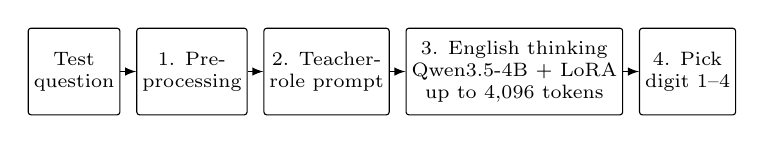
\begin{tikzpicture}[font=\scriptsize, node distance=2mm,
    b/.style={draw, rounded corners=1pt, align=center, inner sep=2pt, minimum height=11mm}, >=latex]
  \node[b] (a) {Test\\question};
  \node[b, right=of a] (p) {1. Pre-\\processing};
  \node[b, right=of p] (b) {2. Teacher-\\role prompt};
  \node[b, right=of b] (c) {3. English thinking\\Qwen3.5-4B + LoRA\\up to 4,096 tokens};
  \node[b, right=of c] (d) {4. Pick\\digit 1--4};
  \draw[->] (a) -- (p); \draw[->] (p) -- (b); \draw[->] (b) -- (c); \draw[->] (c) -- (d);
\end{tikzpicture}
\caption{The pipeline of the final system.}\label{fig:pipeline}
\end{figure}

\para{1. Preprocessing.} The text is first converted to the standard Unicode form (NFC), so that the same word is always stored in the same way. We then remove zero-width non-joiners, invisible characters left over from old Sinhala fonts, but keep zero-width joiners, which Sinhala needs to form some letters. The question is not translated, so the model reads the original Sinhala.

\para{2. Prompt.} We build a single prompt with no worked examples. Its English instructions cast the model as an expert Sri Lankan teacher of the subject, ask it to think step by step in English, and ask it to end with ``Answer: <number>'', while the question and options stay in Sinhala. Section~\ref{sec:prompting} describes the prompt further.

\para{3.1 LoRA adapter.} This stage uses Qwen3.5-4B with our LoRA adapter, which was trained before inference on Sinhala multiple-choice questions (Section~\ref{sec:data}) and then merged into the model, where it accounts for 30.5M parameters. Training teaches only the answer digit and not the reasoning, so the model is never taught to stop after a digit and can still reason at length (Section~\ref{sec:training}).

\para{3.2 English reasoning.} The model writes its reasoning inside Qwen's thinking block, using greedy decoding with at most 4,096 new tokens.

\para{4. Answer selection.} We remove any answer the model stated, append ``Answer:'', and read the probabilities of the digits 1--4 at that position. The most probable digit becomes the answer, so every question receives one valid answer even when the reasoning was cut off at the token limit.

\para{Why this approach.} This system gave our best result. Across the four phases we tried about 70 configurations: 3 small models, 59 inference-time conditions, 6 Gemma adapters and 4 Qwen systems. Of the 7 full systems compared on screening set 2, this one scored highest (59.7\%; Table~\ref{tab:phase2}). Each of its parts came out of one phase: English reasoning over the original Sinhala was the most reliable gain without training, Qwen3.5-4B was the largest single gain among the full systems, and the adapter raised validation accuracy while staying within the 8B limit. Section~\ref{sec:results} reports all the experiments and their results.

\section{Models}\label{sec:params}
Our final system uses two models, Qwen3.5-4B and our LoRA adapter, and only these two are loaded at inference and count towards the 8B limit. Claude Sonnet 5.5 was used solely to create training data. Table~\ref{tab:models} in Appendix~\ref{app:tables} lists every model we used, including those used only in experiments. We used no embedding models, rerankers or teacher models.

\para{Parameter count of the final system: 4.24B.} We load the text model of Qwen3.5-4B (4,205,751,296 parameters) together with the adapter (30,474,240). Merging adds no new parameters, so the loaded model has 4.21B, but we report 4.24B because the rules count LoRA towards the total. The full checkpoint, which includes a vision encoder we do not load, has 4,659,865,088 parameters. Either count is within 8B, and nothing else runs at inference. Section~\ref{sec:results} explains why each model was chosen.

\section{Data}\label{sec:data}
We used two kinds of data. The LoRA adapter was trained on two sources of Sinhala multiple-choice questions, while evaluation relied on the Sinhala MMLU shared-task data provided by the organisers, on which we never trained. Table~\ref{tab:data} in Appendix~\ref{app:tables} lists all the data, with sources and preprocessing.

\subsection{Global-MMLU Sinhala}
Global-MMLU \citep{singh2025globalmmlu} is a multilingual version of the English MMLU benchmark covering 57 subjects, and its Sinhala version was created by translating the MMLU questions. Its translation quality is limited: \citet{pramodya2025sinhalammlu} found the translated questions less natural than native Sinhala ones. We use its 14,324 questions as released, and Appendix~\ref{app:tables} gives a detailed description.

\subsection{\sinmulu{}}\label{sec:sinmulu}
\sinmulu{} is our own collection of Sinhala multiple-choice questions from Sri Lankan exams, which we built for this task in five steps.

\para{Step 1: Collecting the papers.} We collected 3,486 exam-paper PDFs from e-Thaksalawa (\url{https://e-thaksalawa.moe.gov.lk}), the official e-learning portal of Sri Lanka's Ministry of Education, which hosts past papers and term papers for grades 1 to 13. The collection covers G.C.E.\ O/L and A/L papers as well as provincial term tests.

\para{Step 2: Transcribing.} Because most PDFs use legacy Sinhala fonts, their text could not be extracted. We therefore rendered each page as an image, and Claude Sonnet 5.5 read the image and transcribed the questions and options word for word. The papers were processed in batches by several agents working in parallel, using the prompt in Appendix~\ref{app:prompt}.

\para{Step 3: Selecting questions and adding answers.} We kept only Sinhala-medium papers and true multiple-choice questions, skipped calculation-based subjects such as Mathematics, Physics, Accounting and Statistics, and dropped questions that depend on diagrams or could not be read. Answers come from official marking schemes where available, matched to papers by grade, year and province. Otherwise we asked Claude Sonnet 5.5 to generate the answer and kept it only if the model was highly confident, so \textbf{some answers are model-derived}. This step used the same prompt as Step 2.

\para{Step 4: Cleaning.} Validating, de-duplicating and cleaning the records gave 15,355 four-option questions. We did \textbf{not} measure the transcription or label error rate.

\para{Step 5: Removing overlap with the test set.} Real exams repeat questions, so the collection could contain test questions. We therefore compared all 15,355 questions with the 2,238 test questions, without using any answers. Candidates came from character n-gram TF-IDF, each pair was scored with \texttt{difflib} on the question and the choices, and the ranked pairs were reviewed by hand. Two rounds removed 143 and 22 questions, leaving 15,190.

Some similarity remains: 260 test questions still match above 0.7 on the question, and although we judged most of these to be different template questions, 15 score $\geq 0.99$. Because the cleaning rests on manual judgement, it \textbf{does not prove zero leakage}.

\para{Release.} \sinmulu{} is available at \url{https://huggingface.co/datasets/JaniRaviRash-523/sinmulu-si}. Its licence is left as unknown, because the rights to the exam papers remain with their authors and examining bodies.

\subsection{Combined Training Data}
We merged the two sources, after dropping 10 further duplicates from \sinmulu{}, and held out 10\% of each subject for validation (seed 42). This gave 26,675 training and 2,829 validation questions, of which 25,799 and 2,745 remained after skipping questions over 1,024 tokens.

\subsection{Evaluation Data}\label{sec:evaldata}
We created two screening sets to evaluate our systems. The shared-task public dataset has 1,851 Easy questions, all of which we used in phase 1. For phase 2 we first removed 18 near-duplicates of test questions and then split the rest: \textbf{screening set 1} has 280 questions, 20 chosen at random from each of the 14 subjects; 70 questions were set aside as few-shot examples; and the remaining 1,483 questions formed the \textbf{screening 1 confirmation set}.

\textbf{Screening set 2} has 300 questions from the public test set, with 100 each from Easy, Medium and Hard. Since the test set comes without answers, we answered these 300 questions manually from our own knowledge, with the help of AI. We used this set only to compare model results in phases 3 and 4, because no official development set with Easy, Medium and Hard questions is available. These questions and answers were never used anywhere in training.

The full public test set of 2,238 questions was used to produce our predictions.

\section{Implementation Details}\label{sec:impl}
This section describes how we built the final system, in enough detail for another team to rebuild it. Section~\ref{sec:results} covers the other training and prompting experiments.

\subsection{Training}\label{sec:training}
We fine-tuned Qwen3.5-4B with a LoRA adapter \citep{hu2022lora} on the combined data of Section~\ref{sec:data}, using the base model in bf16 with no quantisation, and merged the adapter into the model after training.

The training objective is the answer digit alone. Each training example is a plain multiple-choice prompt (\cond{en\_instr\_nosubject}, Appendix~\ref{app:prompts}) whose reply is pre-filled with ``Answer:\textvisiblespace'', and the loss is $\log P(\text{gold digit})$ at the next token. There is no loss on the question or on an end-of-turn token, so the model is never taught to stop after a digit, which matters because at inference we want it to reason at length. Table~\ref{tab:training} in Appendix~\ref{app:details} gives the settings.

\subsection{Prompting}\label{sec:prompting}
Our experiments covered many prompts: Sinhala and English instructions, subject names and teacher roles, few-shot examples, cloze scoring, reasoning in Sinhala and in English, translated and bilingual input, and instructions for negated questions (Section~\ref{sec:results}). Appendix~\ref{app:prompts} lists all of them under the names we used.

Our final system uses \cond{cot\_en\_role\_think}, whose exact text is given in Appendix~\ref{app:finalprompt}. It has no system prompt and no few-shot examples. Its instructions are in English and the model also reasons in English, while the question and options stay in Sinhala.

\subsection{Inference and Answer Selection}
Decoding is greedy, with at most 4,096 new tokens, length-sorted batches of 48, left padding and seed 42.

We read the answer from the model's probabilities rather than by parsing its text, in four steps. First, we cut any stated ``Answer: N'' from the reasoning. Second, we add \texttt{</think>} if the thinking block was not closed, because this special token disappears when decoding. Third, we append \verb|\n\nAnswer: |, which must end with the space or the digit will not be the next token (Section~\ref{sec:prefill}). Finally, we take the most probable of the four digit tokens as the answer.

No ensemble, voting, self-consistency or fallback rule is used, and reasoning that hits the token limit is scored in the same way.

\section{Compute, APIs and Costs}\label{sec:compute}
This section covers all stages of the work, from data creation to final inference, and Appendix~\ref{app:tables} gives the full table.

\para{Data creation.} We created \sinmulu{} with Claude Sonnet 5.5 (medium effort) through a Claude Code subscription, processing 3,486 PDFs. Token and call counts were not recorded, because Claude was used through a subscription.

\para{Experiments and training.} Phase 1 ran on a free Colab T4 GPU at no cost, and its hours were not recorded. Phase 2 took about 13.5 GPU-hours on an RTX~3090, and phases 3 and 4 took about 40 GPU-hours on RTX~3090, RTX 5000 Ada, L40 and A100 GPUs. These 40 hours include the final LoRA training (8.8 h on an RTX~3090) and the final inference on the test set (about 5 h on an A100 40 GB). Phases 2 to 4 ran on rented RunPod GPUs, for a total of about 53.5 GPU-hours.

\para{Costs.} We spent USD 15 on RunPod to rent GPUs. This does not include the Claude Code subscription.

\para{Minimum hardware.} The final system needs one GPU with bf16 support and 24 GB of memory, because generation with batch 48 uses about 24 GB. Smaller GPUs also work, though more slowly, since a batch that runs out of memory is split. The test set takes about 5 h on one A100 40 GB.

\section{Experiments and Results}\label{sec:results}
We ran our experiments in four phases, a logical division in which each phase answers one question and its result leads to the next (Table~\ref{tab:phases} in Appendix~\ref{app:details}). Section~\ref{sec:effects} brings the results together, and Appendix~\ref{app:details} gives the details. Our final system ranked 11th on the leaderboard, with a Macro Avg of 57.58.

\para{Validation setup.} Each phase used different data (Section~\ref{sec:evaldata}). Phase 1 used all 1,851 questions of the shared-task public dataset, and phase 2 used screening set 1 before confirming the best conditions on the screening 1 confirmation set. For phases 3 and 4 we had no labelled Medium or Hard data, so we compared full prediction files on screening set 2. Scores on this set are optimistic and are not independent estimates (95\% interval about $\pm$5.7 points overall, $\pm$10 per level). Adapters were also validated on held-out parts of their own training data, using the digit prompt.

\subsection{Phase 1: Small-Model Scouting}
Models of 1B or less leave most of the 8B budget free and run on a free Colab T4, which made them the cheapest way to test the pipeline end to end and to see whether such small models carry any signal on Sinhala. We ran Gemma-3-1B-it, Qwen3-0.6B and Llama-3.2-1B-Instruct on all 1,851 questions of the shared-task public dataset. All three were at chance (25.6--26.6\%; Table~\ref{tab:small}), so we moved to the 4B class, and reviewing these runs also uncovered three scoring bugs. Given the time available we chose Gemma-3-4B-it, because Gemma's tokenizer gives prompts about three times shorter than the others.

\subsection{Phase 2: Inference-Time Study}\label{sec:phase2}\label{sec:prefill}
Before spending GPU time on training, we wanted to know what a fixed 4B model can do with prompting and scoring alone. These methods need no extra data, and they give fine-tuning a baseline. We tested 59 conditions on Gemma-3-4B-it, covering prompt wording, scoring methods, reasoning, translation and ensembles. All were run on screening set 1, and the four best valid conditions then went to the screening 1 confirmation set together with the baseline. A rule written down in advance decided adoption: a gain of at least 1 point with Holm-corrected exact McNemar $p<0.05$. Later follow-ups needed $+2$ points on screening set 1 to be confirmed.

Reasoning in English over the Sinhala question was the largest gain. With a teacher role (\cond{cot\_en\_role}), it raised accuracy from 38.2\% to 45.6\% on the screening 1 confirmation set (+7.4 points, 95\% CI [+4.6, +10.3], Holm-corrected $p = 1.2\times10^{-6}$). This is at the level the SinhalaMMLU paper reports for Qwen2.5-72B-chat on Easy questions (45.11\%), although the question sets differ, and no other condition was confirmed above it (Table~\ref{tab:phase1}).

Two results from screening set 1 did not replicate: worked examples fell from 50.7\% to 44.8\%, and Sinhala reasoning from 43.2\% to 36.8\%. This is why we took decisions on the screening 1 confirmation set only. We also found and fixed a scoring pitfall: the answer digit follows a separate space token, so the reply must be pre-filled with a trailing space (Appendix~\ref{app:details}).

\subsection{Phase 3: Fine-Tuning}\label{sec:phase3}
Prompting cannot add knowledge the model lacks, and culture-specific knowledge is the hardest part of SinhalaMMLU. A small adapter can add Sinhala exam knowledge while staying well within the 8B limit, so we trained 6 LoRA adapters on Gemma-3-4B-it, using Global-MMLU Sinhala or \sinmulu{} with different ranks and numbers of epochs.

Real exam questions helped far more than translated ones: validation accuracy rose from 40.9\% to 47.1\% on \sinmulu{}, but only from 40.1\% to 41.5\% on Global-MMLU (Table~\ref{tab:adapters}). However, the gain did not reliably carry over to reasoning prompts. On screening set 2, the Gemma adapters scored 50.3\% and 49.3\% against 47.3\% for the base model, which is within the noise (Table~\ref{tab:phase2}).

\subsection{Phase 4: Stronger Base Model}\label{sec:phase4}
On Gemma, no prompt variant was confirmed above English reasoning and adapters stayed within the noise, which left the base model as the remaining lever. Qwen3.5-4B is in the same size class, is newer, was trained for long reasoning, and has a thinking mode. We moved to it with the same prompt, then added a LoRA adapter trained on the combined data, whose validation accuracy rose from 44.4\% to 54.8\%, and finally turned on thinking mode.

Moving from Gemma to Qwen gave +7.4 points (McNemar $p=0.04$), and the final system beat submission 2 by +12.4 ($p=0.001$). The adapter made no measurable difference on screening set 2 (55.0 vs 54.7, $p=1.0$), while thinking mode added +4.7 ($p=0.17$), mostly on Hard questions (+8). A subject-aware prompt lost 12 points, because fewer of its reasoning texts stated an answer. The leaderboard Macro Avg is 2.1 points below the screening set 2 score, as expected after selecting on that set.

\subsection{Effect of Each Component}\label{sec:effects}
Table~\ref{tab:effects} in Appendix~\ref{app:details} brings the four phases together. Two changes gave clear gains, the adapter helped mainly on its own validation data, and most other methods gave no gain.

\section{Analysis and Limitations}\label{sec:limits}
This section examines where our systems fail, what limits our results, and what we would do next. Results by level and subject come from the final system, whereas results by question type come from the phase-2 Gemma system.

\subsection{Error Analysis}
\para{Difficulty levels.} On the leaderboard, Hard is our strongest level (65.77), followed by Easy (54.67) and Medium (52.30). It is unusual for the hardest level to score highest, and we did not investigate why.

\para{Subjects.} On screening set 2, the final system is strongest on social science (76\%) and STEM (73\%), and weakest on humanities (50\%; religion, art, dance, music) and Sinhala language (44\%). In phase 2, English reasoning helped content subjects most (Geography +17.8, Health +14.4) but not language- or culture-bound subjects (Sinhala $-$2.3, Dancing $-$13.4; Appendix~\ref{app:subjects}), which suggests that reasoning in English loses information when the question is about Sinhala itself.

\para{Unfinished reasoning.} This is the biggest factor in the final system. Questions whose reasoning stated an answer are 73.4\% correct, against 42.0\% when the reasoning hit the 4,096-token limit, which happened on 44\% of questions. The gap is largest on Easy questions (75.8\% vs 31.6\%), where the model over-thinks culture-specific recall questions.

\para{Question types.} English reasoning helps negated questions most (+12.7 points), while sub-option, fill-in-the-blank and numeric questions remain the weakest types (Table~\ref{tab:types}).

\subsection{Limitations}
\begin{list}{--}{\leftmargin=1em\itemindent=0pt\itemsep=1pt\parsep=0pt\topsep=2pt}
\item The final system was selected on test questions.
\item All development data is Easy, so gains may not transfer to Medium and Hard.
\item \sinmulu{} has transcription and model-derived labelling errors that we could not measure, and no per-record flag for answer source.
\item Residual near-duplicates mean that zero leakage is not proven.
\item Long reasoning is slow and often cut off.
\item Adapters are validated with a digit prompt but used with a reasoning prompt, and the two do not always move together.
\item GPU type changes scores, because bf16 rounding changes greedy reasoning: the same Gemma system scored 47.3\% and 44.3\% on screening set 2 on two GPU types, so a reproduction on other hardware will differ in some answers.
\item Some raw follow-up outputs were lost with a terminated pod, although the numbers had already been logged.
\end{list}

\subsection{What We Would Try Next}
Choosing the system on test questions is our largest weakness, so we would first build a labelled Medium/Hard development set from our own O/L and A/L papers. Since unfinished reasoning is our largest error source, we would then add a token budget to shorten thinking. Finally, because the adapter did not clearly help reasoning prompts, we would train it on short English rationales, including negated questions.

\section{Reproducibility Checklist}\label{sec:reproduction}
\begin{list}{}{\leftmargin=1.4em\itemindent=-1.4em\itemsep=2pt\parsep=0pt\topsep=2pt}\raggedright
\item \ticked{} All code, the inference script, requirements.txt and predictions.jsonl are in SinhalaMMLU-SharedTask/team-sinbotics
\item \unticked{} All trained models and adapters are in SinhalaMMLU-SharedTask/team-sinbotics-<model> repositories
\item \ticked{} The inference script reads the dataset from the DATA\_REPO line and runs from start to finish in a fresh environment
\item \ticked{} All data used is released or linked in Section~\ref{sec:data}
\item \unticked{} Every model, API and cost is listed in Sections~\ref{sec:params} and~\ref{sec:compute}
\item \ticked{} The report file is named SinhalaMMLU2026\_team-sinbotics\_SystemReport.pdf
\end{list}

\smallskip
\section{Use of AI Assistants}
Claude Code (Claude Opus 5.5) wrote and ran most of the code and experiments, prepared the submission, and drafted this report from our logs, while the team directed the work and made the decisions. Claude Sonnet 5.5 created \sinmulu{} (Section~\ref{sec:data}), and AI also helped us answer the questions of screening set 2 (Section~\ref{sec:evaldata}). No AI assistant or API is used at inference.

\section{Declaration: No Sinhala MMLU Data Used for Training}\label{sec:declaration}
\ticked{} We confirm that no Sinhala MMLU data was used, directly or indirectly, to train, fine-tune or otherwise build any part of our system. ``Sinhala MMLU data'' means any data from the Sinhala MMLU benchmark in any form, including but not limited to the shared task development and test sets, the original SinhalaMMLU dataset, and any copies, translations, paraphrases, or derived or synthetic versions of its questions or answers. ``Any part of our system'' means every component, including but not limited to model weights, adapters, prompts and few-shot examples.

Appendix~\ref{app:decl} states which data we used for validation only, and how, with our overlap check.

\bibliography{references}

\onecolumn
\appendix
\renewcommand{\thesection}{\Alph{section}}
\section{Task Rules and Compliance}\label{app:rules}

\begin{center}\captionsetup{type=table}
\small
\caption{Task rules and how our system complies.}\label{tab:rules}
\begin{tabularx}{\columnwidth}{@{}L{0.36\columnwidth}Y@{}}
\toprule
Rule & Our system \\
\midrule
$\leq$ 8B parameters at inference & 4.24B, one model (Section~\ref{sec:params}) \\
Open weights before 1 Oct 2026 & Qwen3.5-4B: 27 Feb 2026, Apache-2.0 \\
No retrieval & none; no few-shot examples either \\
Closed APIs only for training data, disclosed & Claude Sonnet 5.5 for \sinmulu{} only (Section~\ref{sec:data}) \\
No tuning on test questions & none trained on; systems were compared on screening set 2 (Section~\ref{sec:results}) \\
Reproducible from code & greedy decoding, pinned versions, model revision (Section~\ref{sec:reproduction}) \\
\bottomrule
\end{tabularx}
\end{center}

\section{Full Model, Data and Compute Tables}\label{app:tables}

\begin{center}\captionsetup{type=table}
\small
\caption{All models used, grouped by purpose. The final system is highlighted. HF = huggingface.co.}\label{tab:models}
\begin{tabularx}{\textwidth}{@{}L{0.25\textwidth}L{0.25\textwidth}L{0.06\textwidth}YL{0.07\textwidth}L{0.13\textwidth}@{}}
\toprule
Model & HF link or provider & Params & Role & Used at inference? & Fine-tuned by you? \\
\midrule
\multicolumn{6}{@{}l}{\best{Final system}} \\
\best{Qwen/Qwen3.5-4B} (rev.\ 851bf6e8) & HF: Qwen/Qwen3.5-4B & \textbf{4.21B} & base model & \textbf{Yes} & \textbf{Yes, LoRA} \\
\best{Our LoRA adapter} (rank 16) & HF: \repo, \texttt{adapter/} & \textbf{30.5M} & merged into the base model & \textbf{Yes, merged} & \textbf{Yes, trained by us} \\
\midrule
\multicolumn{6}{@{}l}{\emph{Data creation}} \\
Claude Sonnet 5.5 \citep{anthropic2026sonnet} & Anthropic, via Claude Code & closed & transcribing exam papers and labelling answers for \sinmulu{} & No & No \\
\midrule
\multicolumn{6}{@{}l}{\emph{Experiments only (not in the final system)}} \\
google/gemma-3-4b-it & HF: google/gemma-3-4b-it & 4.30B & main model of phases 2 and 3 & No & Yes, LoRA (6 adapters) \\
google/gemma-3-4b-pt & HF: google/gemma-3-4b-pt & 4.30B & phase-2 reference & No & No \\
google/gemma-3-1b-it & HF: google/gemma-3-1b-it & 1.0B & phases 1 and 2, small-model reference & No & No \\
Qwen/Qwen3-0.6B & HF: Qwen/Qwen3-0.6B & 0.6B & phase 1, small-model scouting & No & No \\
meta-llama/Llama-3.2-1B-Instruct & HF: meta-llama/Llama-3.2-1B-Instruct & 1.2B & phase 1, small-model scouting & No & No \\
facebook/nllb-200-distilled-600M \citep{nllb2022} & HF: facebook/nllb-200-distilled-600M & 0.62B & phase-2 translation & No & No \\
google/madlad400-3b-mt \citep{kudugunta2023madlad} & HF: google/madlad400-3b-mt & 2.94B & phase-2 translation & No & No \\
\bottomrule
\end{tabularx}
\end{center}

Gemma-3-4B-it is efficient on Sinhala (3.04 tokens per word). Qwen3.5-4B is a hybrid of 24 Gated-DeltaNet linear-attention layers and 8 full-attention layers, and costs 4.78 tokens per word.

\clearpage
\begin{center}\captionsetup{type=table}
\small
\caption{All data used. HF = huggingface.co.}\label{tab:data}
\begin{tabularx}{\textwidth}{@{}L{0.16\textwidth}L{0.26\textwidth}L{0.08\textwidth}L{0.07\textwidth}YL{0.2\textwidth}@{}}
\toprule
Dataset & Source or link & Language & Size & How it was used & Preprocessing \\
\midrule
Shared-task public dataset & organisers & Sinhala & 1,851 (Easy) & validation only; 70 as a few-shot pool in phase 2 & 18 near-duplicates of test questions removed; 1 label fixed \\
Public test set & organisers & Sinhala & 2,238 & predictions; 300 questions as screening set 2 for system comparison & zero-width non-joiners removed \\
Global-MMLU si \citep{singh2025globalmmlu} & HF: datasets/CohereLabs/Global-MMLU (si, rev.\ 0e619dbe) & Sinhala (translated) & 14,324 & LoRA training (12,926) and validation (1,398) & test and dev splits merged; 3 items with an empty option dropped \\
\sinmulu{} (ours) & HF: datasets/JaniRaviRash-523/sinmulu-si; 3,486 exam-paper PDFs & Sinhala & 15,180 & LoRA training (13,749) and validation (1,431) & 165 test overlaps and 10 duplicates removed \\
\textbf{Combined (final adapter)} & union of the two above & Sinhala & 29,504 & training 26,675 and validation 2,829 (10\% per subject, seed 42) & questions over 1,024 tokens skipped (25,799 and 2,745 used) \\
\bottomrule
\end{tabularx}
\end{center}

\para{Global-MMLU Sinhala.} Global-MMLU \citep{singh2025globalmmlu} extends the English MMLU benchmark to 42 languages, and paid professional and community annotators checked the translation quality. We used its Sinhala configuration (\texttt{CohereLabs/Global-MMLU}, \texttt{si}, revision 0e619dbe, Apache-2.0), which covers 57 subjects. We merged its test split (14,042 questions) and dev split (285 questions), and dropped 3 questions with an empty option, leaving 14,324. We then held out 10\% of each subject for validation, which gave 12,926 training and 1,398 validation questions.

Global-MMLU is a larger source than our own exam questions, but a less natural one. \citet{pramodya2025sinhalammlu} sampled 100 translated STEM questions from it and 100 native SinhalaMMLU questions, and two Sinhala-speaking annotators rated their naturalness. The translated questions scored 71.07 out of 100, against 97.30 for the native ones. For example, the term ``plasmolysis'' was written as a sound-alike of the English word, not as the standard Sinhala technical term.

\para{Shared-task data.} We fixed one invalid training label (Geography, question 64), and copied the inconsistent subject strings of the test files verbatim into submissions. We removed the zero-width non-joiner, which appears in 357 test items but only 29 training items.

\begin{center}\captionsetup{type=table}
\small
\caption{Compute, APIs and costs. GPU hours are approximate.}\label{tab:compute}
\begin{tabularx}{\textwidth}{@{}YL{0.25\textwidth}L{0.16\textwidth}L{0.15\textwidth}L{0.09\textwidth}@{}}
\toprule
Stage & Hardware or API & Platform & GPU hours or usage & Cost (USD) \\
\midrule
Data creation (\sinmulu{}) & Claude Sonnet 5.5, medium effort & Claude Code subscription & 3,486 PDFs & not listed \\
Phase 1: small-model scouting & 1$\times$ T4 & Colab (free) & not recorded & 0 \\
Phase 2: inference-time study & 1$\times$ RTX~3090 & RunPod & 13.5 GPU-h & in total \\
Phases 3 and 4: training and experiments & RTX~3090, RTX 5000 Ada, L40, A100 & RunPod & 40 GPU-h & in total \\
\quad of which final LoRA training & 1$\times$ RTX~3090 & RunPod & 8.8 h & \\
\quad of which final inference & 1$\times$ A100 40 GB & RunPod & 5 h & \\
\textbf{Total (RunPod rental; excludes the Claude Code subscription)} & & & \textbf{53.5 GPU-h} & \textbf{15} \\
\bottomrule
\end{tabularx}
\end{center}

\section{Final Prompt}\label{app:finalprompt}
The user turn of \cond{cot\_en\_role\_think}, with no system prompt:

\smallskip
{\footnotesize\ttfamily\raggedright\noindent
You are an expert Sri Lankan teacher of \{subject\}.\\
The following is a multiple choice question in Sinhala about \{subject\}.\\
Think step by step in English, then choose the correct or most suitable answer from the options 1, 2, 3, 4.\\
End your reply with "Answer: <number>".\\[2pt]
Question: \{Sinhala question\}\\
1. \{option 1\}\\
2. \{option 2\}\\
3. \{option 3\}\\
4. \{option 4\}\par}

\smallskip\noindent\{subject\} is the English subject name from the test file. The prompt is rendered with Qwen's chat template, with \texttt{enable\_thinking=True} and a fixed template date.

\section{Declaration Details}\label{app:decl}
\para{Data used for validation only.} We used two kinds of Sinhala MMLU data for validation, and neither was used for training.

\begin{list}{--}{\leftmargin=1em\itemindent=0pt\itemsep=1pt\parsep=0pt\topsep=2pt}
\item \emph{Shared-task public dataset.} We used it to choose prompts and methods in phases 1 and 2. Its 70 few-shot questions were used in phase-2 experiments only, and the final system has no few-shot examples and no dataset question in its prompt.
\item \emph{Screening set 2.} We scored full test-prediction files on these 300 public test questions, using answers we prepared manually with the help of AI, to choose between the systems of phases 3 and 4. This comparison selected our final system.
\end{list}

\para{Overlap check.} \sinmulu{} comes from the same kind of exam papers as Sinhala MMLU. After the cleaning of Section~\ref{sec:sinmulu}, no test or public question appears in \sinmulu{} with the same question text and at least three of the same options. However, 10 test questions and 1 public question have the same question text with different options, and near-duplicates remain, so zero leakage is not proven.

\section{Experiment Details}\label{app:details}

\begin{center}\captionsetup{type=table}
\footnotesize
\caption{The four experimental phases.}\label{tab:phases}
\begin{tabularx}{\textwidth}{@{}L{0.14\textwidth}L{0.3\textwidth}L{0.2\textwidth}Y@{}}
\toprule
Phase & Question, and why we asked it & Models & Main result \\
\midrule
\textbf{1. Small-model scouting} & Do models of 1B or less have any signal? They run on free GPUs, so they also test the whole pipeline cheaply. & Gemma-3-1B-it, Qwen3-0.6B, Llama-3.2-1B-Instruct & All at chance, so a larger model is needed. Gemma's tokenizer is about 3 times more efficient on Sinhala. Three scoring bugs found. \\
\textbf{2. Inference-time study} & What can a 4B model gain with no training? This is cheap, needs no extra data, and sets the baseline. & Gemma-3-4B-it, with NLLB and MADLAD for translation & English reasoning +7.4 points. Translation, calibration, few-shot, cloze, self-consistency and ensembles give no confirmed gain beyond it. \\
\textbf{3. Fine-tuning} & Can Sinhala exam data add knowledge that prompts cannot? & Gemma-3-4B-it + 6 LoRA adapters & Validation +6.2 points on \sinmulu{}, but the gain on reasoning prompts stays within noise. \\
\textbf{4. Stronger base model} & Does a newer model built for long reasoning beat further work on Gemma? & Qwen3.5-4B, LoRA, thinking mode & +7.4 points over Gemma; final system 59.7 on screening set 2, 57.58 on the leaderboard. \\
\bottomrule
\end{tabularx}
\end{center}

\begin{center}\captionsetup{type=table}
\footnotesize
\caption{Phases 3 and 4 on screening set 2, 300 test questions (accuracy, \%; about $\pm$5.7 overall, $\pm$10 per level), and the leaderboard. S2 is submission 2.}\label{tab:phase2}
\begin{tabularx}{\columnwidth}{@{}Yrrrr@{}}
\toprule
System & Easy & Med. & Hard & All \\
\midrule
Gemma, \cond{cot\_en\_role} (S2) & 49 & 46 & 47 & 47.3 \\
+ LoRA Global-MMLU & 53 & 51 & 47 & 50.3 \\
+ LoRA \sinmulu{}, 2 epochs & 49 & 53 & 46 & 49.3 \\
Qwen, \cond{cot\_en\_role} & 59 & 48 & 57 & 54.7 \\
Qwen + subject hints, NOT rule & 46 & 46 & 36 & 42.7 \\
Qwen + combined LoRA & 56 & 53 & 56 & 55.0 \\
\textbf{+ thinking, 4,096 tokens (final)} & \textbf{59} & \textbf{56} & \textbf{64} & \best{59.7} \\
\midrule
\textbf{Final, leaderboard} & \textbf{54.67} & \textbf{52.30} & \textbf{65.77} & \best{57.58} \\
\bottomrule
\end{tabularx}
\end{center}

\begin{center}\captionsetup{type=table}
\footnotesize
\caption{Effect of each component, in accuracy points against its reference. Conf.: screening 1 confirmation set. Set 1: screening set 1. Set 2: screening set 2 (test questions). Val.: adapter validation set.}\label{tab:effects}
\begin{tabularx}{\columnwidth}{@{}Yrl@{}}
\toprule
Component & Effect & Evidence \\
\midrule
\multicolumn{3}{@{}l}{\emph{Clear gains}} \\
English reasoning, teacher role & +7.4 & Conf., $p_\text{H}=1.2\text{e-}6$ \\
Gemma to Qwen3.5-4B & +7.4 & Set 2, $p=0.04$ \\
\midrule
\multicolumn{3}{@{}l}{\emph{Gains that are not significant}} \\
Thinking mode & +4.7 & Set 2, $p=0.17$ \\
Ensemble of 3 reasoning prompts & +1.1 & Conf., $p=0.31$ \\
\midrule
\multicolumn{3}{@{}l}{\emph{Clear on validation, not on reasoning prompts}} \\
LoRA, \sinmulu{}, on Gemma & +6.2 & Val. \\
LoRA, combined data, on Qwen & +10.4 & Val.; Set 2 +0.3 \\
\midrule
\multicolumn{3}{@{}l}{\emph{No gain, or worse}} \\
Option-order averaging of reasoning & +0.7 & Set 1, $p=0.88$ \\
Bilingual input, MADLAD & +0.4 & Set 1, $p=1.00$ \\
Negation check & $-$1.3 & Conf., $p=0.33$ \\
Self-consistency & $-$1.4 & Set 1 \\
Negation-consistency chain & $-$1.4 & Set 1, $p=0.74$ \\
Contextual calibration & $-$3.2 & Set 1, $p=0.16$ \\
English-only input, MADLAD & $-$4.6 & Set 1, $p=0.25$ \\
Cloze scoring & $-$6.1 & Set 1, $p=0.13$ \\
Judge each option in turn & $-$10.0 & Set 1, $p=0.001$ \\
\bottomrule
\end{tabularx}
\end{center}

\begin{center}\captionsetup{type=table}
\small
\caption{Training settings of the final adapter.}\label{tab:training}
\begin{tabularx}{\columnwidth}{@{}L{0.24\columnwidth}Y@{}}
\toprule
Setting & Value \\
\midrule
LoRA & rank 16, $\alpha = 32$, dropout 0.05 \\
Targets & attention and MLP projections, and the linear-attention projections of all 32 text layers \\
Optimiser & AdamW, learning rate $10^{-4}$, cosine schedule with 3\% warm-up, weight decay 0, gradient clipping 1.0 \\
Epochs & 1 (807 steps) \\
Batching & 32 questions per step, micro-batches of at most 12,288 padded tokens \\
Max length & 1,024 tokens \\
Quantisation & none \\
Seed & 42 \\
Libraries & torch 2.8.0, transformers 5.18.0 \citep{wolf2020transformers}, peft 0.21.1 \citep{mangrulkar2022peft}, accelerate 1.15.0, flash-linear-attention 0.4.0 \citep{yang2024fla}, causal-conv1d 1.7.0 \\
\bottomrule
\end{tabularx}
\end{center}

\begin{center}\captionsetup{type=table}
\small
\caption{Phase 1 on 1,851 questions ($\pm$2.0). Label mass: probability on the four digits. Fertility: tokens per Sinhala word.}\label{tab:small}
\begin{tabularx}{\columnwidth}{@{}Yrrr@{}}
\toprule
Model & Acc. & Label mass & Fertility \\
\midrule
Qwen3-0.6B & 25.6 & 0.010 & 8.66 \\
Gemma-3-1B-it & 26.6 & 0.984 & 2.96 \\
Llama-3.2-1B-Instruct & 25.6 & 0.873 & 10.74 \\
\bottomrule
\end{tabularx}
\end{center}

\para{Scoring pitfall: the pre-fill and the space token.} Our first run on Gemma had a mean label mass, the total probability on the four digits, of only 0.05. Gemma starts its reply with a phrase or ``**'', and it encodes `` 2'' as a space token and a digit, so after ``Answer:'' the next token is the space. Pre-filling the reply with a trailing space raised the label mass to 1.000 (Table~\ref{tab:prefill}). We therefore report label mass for every run, and trust a condition only if it is at least 0.5.

\begin{center}\captionsetup{type=table}
\small
\caption{Answer pre-fill probe, Gemma-3-4B-it, 40 questions. \textvisiblespace{} marks the trailing space.}\label{tab:prefill}
\begin{tabularx}{\columnwidth}{@{}Yr@{}}
\toprule
Text appended after the chat prompt & Label mass \\
\midrule
nothing & 0.053 \\
``\si{පිළිතුර}:'' (Sinhala for ``Answer:'') & 0.000 \\
\textbf{``\si{පිළිතුර}:\textvisiblespace''} & \textbf{1.000} \\
\textbf{``Answer:\textvisiblespace''}, English instructions & \textbf{1.000} \\
\bottomrule
\end{tabularx}
\end{center}

\begin{center}\captionsetup{type=table}
\small
\caption{Phase 2, Gemma-3-4B-it on Easy questions of the shared-task public dataset (accuracy, \%). Conf.: 1,483 questions ($\pm$2.5). Gain: confirmation accuracy minus the baseline. Follow-ups at 1,024 tokens have reference 48.9 on screening set 1.}\label{tab:phase1}
\begin{tabularx}{\columnwidth}{@{}Yrrrl@{}}
\toprule
Condition & Set 1 & Conf. & Gain & $p_\text{H}$ \\
\midrule
Paper prompt, baseline & 37.5 & 38.2 & -- & -- \\
Teacher role in Sinhala & 43.6 & -- & & \\
3-shot, same subject & 42.5 & -- & & \\
Contextual calibration \citep{zhao2021calibrate} & 34.3 & -- & & \\
Cloze scoring of option texts & 31.4 & -- & & \\
4 option orders & 38.6 & -- & & \\
Reasoning in Sinhala & 43.2 & 36.8 & $-$1.3 & \\
Reasoning in English (\cond{cot\_en}) & 47.9 & 44.9 & +6.7 & 1.7e-5 \\
+ 2 worked examples & 50.7 & 44.8 & +6.6 & 3.2e-5 \\
Ensemble \cond{cot\_en} + Sinhala reasoning & 49.3 & 44.0 & +5.9 & 3.8e-5 \\
\textbf{+ teacher role} (\cond{cot\_en\_role}) & \textbf{48.2} & \best{45.6} & \textbf{+7.4} & \textbf{1.2e-6} \\
\midrule
\multicolumn{5}{@{}l}{\emph{Follow-ups to \cond{cot\_en\_role}}} \\
Bilingual input, MADLAD & 49.3 & -- & & \\
Translate first (no second model) & 50.4 & -- & & \\
Self-consistency, 5 samples \citep{wang2023self} & 47.5 & -- & & \\
Judge each option in turn & 38.9 & -- & & \\
Option-order averaging of reasoning & 49.6 & -- & & \\
Negation check in the prompt & 51.4 & 44.3 & +6.1 & \\
Negation-consistency chain & 47.5 & -- & & \\
Ensemble of 3 reasoning prompts & 50.4 & 46.7 & +8.5 & \\
\bottomrule
\end{tabularx}
\end{center}

\para{Reasoning length.} At 512 tokens, 79.3\% of the texts on screening set 1 stated an answer; from 768 tokens up, the limit no longer changed any prediction. On the longer test questions, 512 tokens gave only 62.4\% stated answers and 1,024 gave 99.1\%, so submission~2 used 1,024 tokens.

\para{Confirmation details.} Against the baseline, \cond{cot\_en\_role} is right on 283 questions where the baseline is wrong, and wrong on 173 where it is right. The negation check passed the +2 rule on screening set 1 but fell to 44.3\% on the screening 1 confirmation set. The three-prompt ensemble was only +1.1 over the winner on those questions ($p=0.31$), and we chose it after seeing those results, so it was not adopted.

\para{Adapter details.} Training loss kept falling while validation stopped improving. With reasoning on screening set 1, the base model scored 47.1\%, and the rank-16 \sinmulu{} adapter 46.8\% and 51.4\% after epochs 1 and 2. The final Qwen adapter took 8.8 h on an RTX~3090. Its validation accuracy on 2,745 questions with the digit prompt was 44.4\% at step 0, then 47.4, 49.9, 51.7, 51.7, 52.8, 53.2 and 54.5 at steps 100 to 700, and 54.8\% at step 807.

\begin{center}\captionsetup{type=table}
\small
\caption{Gemma-3-4B-it adapters: validation accuracy (\%) with the digit prompt. Each row has its own validation set, so only compare within a row.}\label{tab:adapters}
\begin{tabularx}{\columnwidth}{@{}Yrrrrr@{}}
\toprule
Training data & Rank & Before & Ep.\ 1 & Ep.\ 2 & Ep.\ 3 \\
\midrule
Global-MMLU si & 16 & 40.1 & 41.5 & -- & -- \\
\sinmulu{} & 16 & 40.9 & 47.1 & 47.3 & 45.8 \\
\sinmulu{}, dropout 0.1 & 8 & 37.5 & 43.8 & 44.4 & -- \\
\bottomrule
\end{tabularx}
\end{center}

\begin{center}\captionsetup{type=table}
\small
\caption{Accuracy (\%) by question type, screening 1 confirmation set.}\label{tab:types}
\begin{tabularx}{\columnwidth}{@{}Yrrrrr@{}}
\toprule
& Neg. & Sub-opt. & Blank & Num. & Plain \\
\midrule
$n$ & 157 & 22 & 104 & 119 & 1,123 \\
Baseline & 37.6 & 27.3 & 28.8 & 35.3 & 39.2 \\
\cond{cot\_en\_role} & \textbf{50.3} & 31.8 & 35.6 & 37.0 & 46.3 \\
Gain & \textbf{+12.7} & +4.5 & +6.8 & +1.7 & +7.1 \\
\bottomrule
\end{tabularx}
\end{center}

\para{Final run.} In the final run, 56.0\% of the reasoning texts stated an answer, and 97.4\% of those agree with the digit we read. The label mass, which is the total probability on the four digits, is 0.999.

\para{Negation and translation.} Translation often loses negation. Of 34 negated questions in screening set 1, the translation kept a negation in only 21 for MADLAD (62\%), 20 for NLLB (59\%) and 19 for self-translation (56\%). On these questions, English reasoning over the original Sinhala scores 58.8\%, against 38.2\% with bilingual input and 29.4\% with English only. A chain that also answers the opposite question hurt too (negated questions fell to 47.1\%), so Gemma decides best when it reasons directly towards one answer.

\para{Reproduction.} The organisers ran our inference script and generated predictions from it. We also checked that the script reproduces the prompts and scoring of all 2,238 questions. On 26 October the phase-2 system was rebuilt from committed code on a new RTX~3090 machine, and all 2,238 test answers matched submission~2.

\clearpage

\section{Prompts}\label{app:prompts}

Shared pieces (Appendix~B of \citep{pramodya2025sinhalammlu}): \textsc{head} = ``\si{පහත දැක්වෙන්නේ බහුවරණ ප්‍රශ්නයකි.}''
(``The following is a multiple choice question.''); \textsc{head-subject} = ``\si{පහත දැක්වෙන්නේ} \{subject\}
\si{සම්බන්ධ බහුවරණ ප්‍රශ්නයකි.}''; \textsc{instr} = ``\si{පහත දැක්වෙන ප්‍රශ්නය සඳහා නිවැරදි හෝ වඩාත්ම ගැළපෙන පිළිතුර
1, 2, 3, 4 පිළිතුරුවලින් තෝරන්න.}'' (``Choose the correct or most suitable answer to the following question from the
answers 1, 2, 3, 4.''); \textsc{body} = ``\si{ප්‍රශ්නය}: \{question\} / 1. \ldots\ / 4. \ldots\ / \si{පිළිතුර}:''.

{\small
\begin{longtable}{p{0.29\linewidth}p{0.65\linewidth}}
\toprule
Name & Text (user turn; ``/'' = line break)\\
\midrule
\endhead
\cond{paper\_nosubject} (A0) & \textsc{head} / \textsc{instr} / / \textsc{body}\\
\cond{paper\_subject\_si} (B1) & \textsc{head-subject} with the Sinhala subject name / \textsc{instr} / / \textsc{body}\\
\cond{paper\_subject\_en} (B2) & as B1 with the English subject name\\
\cond{strict\_nosubject} (B3) & \textsc{head} / \textsc{instr} / ``\si{ඔබේ පිළිතුර ලෙස 1, 2, 3 හෝ 4 යන ඉලක්කම පමණක්
ලියන්න. වෙනත් කිසිවක් ලියන්න එපා.}'' (``Write only the digit 1, 2, 3 or 4 as your answer. Do not write anything else.'')
/ / \textsc{body}\\
\cond{role\_subject\_si} (B4) & ``\si{ඔබ} \{subject\} \si{විෂය පිළිබඳ ප්‍රවීණ ශ්‍රී ලාංකික ගුරුවරයෙකි.}'' (``You are an
expert Sri Lankan teacher of the subject \{subject\}.'') / then B1\\
\cond{en\_instr\_nosubject} (B5) & ``The following is a multiple choice question in Sinhala. / Choose the correct or most
suitable answer from the options 1, 2, 3, 4. / / Question: \{Sinhala question\} / options / Answer:''\\
\cond{letters\_nosubject} (B6) & as A0 with ``A, B, C, D'' in \textsc{instr} and options labelled A.--D.\\
\cond{fewshot$k$\_nosubject} (B7) & $k$ earlier turns (A0 text of an example / ``\si{පිළිතුර}: $d$''), then A0\\
\cond{fewshot3\_subject\_si} & 3 earlier turns in B1 format, then B1\\
\cond{cloze\_nosubject} (C4) & ``\si{පහත දැක්වෙන්නේ ප්‍රශ්නයකි. නිවැරදි පිළිතුර ලියන්න.}'' (``The following is a question.
Write the correct answer.'') / / ``\si{ප්‍රශ්නය}: \{question\} / \si{පිළිතුර}:'' (no options)\\
\cond{cot\_si} (C6) & \textsc{head} / \textsc{instr} / ``\si{පිළිතුර තෝරා ගැනීමට පෙර පියවරෙන් පියවර සිංහලෙන් තර්ක කරන්න.
අවසානයේ ``පිළිතුර: <අංකය>'' ලෙස ලියන්න.}'' (``Before choosing the answer, reason step by step in Sinhala. At the end
write `Answer: <number>'.'') / / question / options\\
\cond{cot\_en} (C7) & ``The following is a multiple choice question in Sinhala. / Think step by step in English, then
choose the correct or most suitable answer from the options 1, 2, 3, 4. / End your reply with ``Answer: <number>''. / /
Question: \{Sinhala question\} / options''\\
\cond{cot\_en\_subject} & as C7 with ``\ldots question in Sinhala about \{English subject\}.''\\
\cond{cot\_en\_role} (phase-2 winner) & ``You are an expert Sri Lankan teacher of \{English subject\}.'' / then
\cond{cot\_en\_subject}\\
\cond{cot\_en\_fewshot2} & 2 earlier turns (C7 text of an example / the model's own correct English reasoning),
then C7\\
\cond{en\_nosubject} (D1--D3) & ``The following is a multiple choice question. / Choose the correct or most suitable
answer from the options 1, 2, 3, 4. / / Question: \{English translation\} / translated options / Answer:''\\
\cond{bilingual\_nosubject} (D4) & ``The following is a multiple choice question in Sinhala, followed by a machine
translation into English. / The translation may contain errors; the Sinhala text is the original. / Choose \ldots /
/ Sinhala: / \si{ප්‍රශ්නය}: \ldots\ / options / / English: / Question: \ldots\ / translated options / Answer:''\\
\cond{si\_q\_en\_opts} (D5) & A0 with the options replaced by their English translations\\
\cond{cot\_en\_role\_think} (\textbf{final system}) & the same text as \cond{cot\_en\_role}, rendered with \texttt{enable\_thinking=True}, at most 4,096 new tokens (Section~\ref{sec:prompting})\\
\cond{cot\_en\_role\_subject\_aware} & \textsc{role-head} / one subject hint (listed below) / ``If the question asks which option is NOT correct (or does not match), choose the false option.'' / \textsc{cot} / / Question: \{Sinhala question\} / options\\
\cond{cot\_en\_role\_bilingual} & \textsc{role-head} / ``The question is given in Sinhala, followed by a machine translation into English. The translation may contain errors; the Sinhala text is the original.'' / \textsc{cot} / / Question (Sinhala): \{Sinhala question\} / options / / Machine translation (English): / Question: \{English translation\} / translated options\\
\cond{cot\_en\_role\_en} & ``You are an expert Sri Lankan teacher of \{subject\}. / The following is a multiple choice question about \{subject\}.'' / \textsc{cot} / / Question: \{English translation\} / translated options\\
\cond{cot\_en\_role\_negcheck} & \textsc{role-head} / ``Before reasoning, state whether the question asks for the correct option or for the option that is NOT correct, does NOT match, or is false. Then think step by step in English and choose the correct or most suitable answer from the options 1, 2, 3, 4. / End your reply with ``Answer: <number>''.'' / / Question: \{Sinhala question\} / options\\
\cond{cot\_en\_role\_each\_option} & \textsc{role-head} / ``Evaluate each of the four options one by one and say whether it is correct or incorrect for this question, thinking in English. Then choose the correct or most suitable answer from the options 1, 2, 3, 4. / End your reply with ``Answer: <number>''.'' / / Question: \{Sinhala question\} / options\\
\cond{cot\_en\_role\_translate\_first} & \textsc{role-head} / ``First translate the question and the four options into English. Then think step by step in English and choose the correct or most suitable answer from the options 1, 2, 3, 4. / End your reply with ``Answer: <number>''.'' / / Question: \{Sinhala question\} / options\\
\cond{cot\_en\_role\_negchain}, turn 1 & \textsc{role-head} / ``Think step by step in English. For each of the options 1, 2, 3, 4, decide whether it is a correct answer to this question. More than one option may be correct. / End your reply with ``Correct options: <numbers separated by commas>''.'' / / Question: \{Sinhala question\} / options\\
\cond{cot\_en\_role\_negchain}, turn 2 & ``Now negate the question: write the opposite question in English (if the question asks which option is correct, the opposite question asks which options are NOT correct, and if it asks which option is NOT correct, the opposite question asks which options are correct). Then think step by step in English and decide for each of the options 1, 2, 3, 4 whether it answers the opposite question. / End your reply with ``Options for the opposite question: <numbers separated by commas>''.''\\
\cond{cot\_en\_role\_negchain}, turn 3 & ``Now use both analyses, the original question with its correct options and the opposite question with its options, to choose the single correct or most suitable answer to the ORIGINAL question from the options 1, 2, 3, 4. Explain briefly in English (at most three sentences), then end your reply with ``Answer: <number>''.''\\
\bottomrule
\end{longtable}}

\noindent The later prompts use two more shared pieces: \textsc{role-head} = ``You are an expert Sri Lankan teacher of \{subject\}. / The following is a multiple choice question in Sinhala about \{subject\}.''; \textsc{cot} = ``Think step by step in English, then choose the correct or most suitable answer from the options 1, 2, 3, 4. / End your reply with ``Answer: <number>''.''

\noindent Subject hints of \cond{cot\_en\_role\_subject\_aware}, by subject group. Sinhala: ``This question tests Sinhala language and literature (grammar, vocabulary, idioms, literary works). Pay close attention to the exact Sinhala wording and spelling of each option.'' Religion: ``Answer according to the teachings of this religion as taught in the Sri Lankan school curriculum.'' History, geography, civics, politics, communication, health: ``Use knowledge of Sri Lanka (history, geography, government and society) as taught in the Sri Lankan school curriculum.'' Science and technology: ``Reason step by step and check facts, units and calculations carefully.'' Business and economics: ``Apply the definitions and principles of the Sri Lankan syllabus and check any calculation.'' Art, dance, drama, music: ``Recall the specific traditional Sri Lankan terms, artists, forms and techniques.''


\section{Screening Results}\label{app:screen}

{\footnotesize\setlength{\tabcolsep}{4pt}
\begin{longtable}{p{0.5ex}lrrrrrr}
\caption{Screening set 1 ($n$=280; chance 27.5\%). Gain = accuracy minus baseline (points);
CI = paired bootstrap 95\% interval of the gain; $p$ = exact McNemar; $p_\text{H}$ = Holm-corrected over the 39
comparisons of the final table; L = mean label mass. All with Gemma-3-4B-it, chat template, one option order, no
calibration, bf16, unless stated.}\label{tab:screen}\\
\toprule
& Condition & Acc. & Gain & CI of gain & $p$ & $p_\text{H}$ & L\\
\midrule
\endfirsthead
\toprule
& Condition & Acc. & Gain & CI of gain & $p$ & $p_\text{H}$ & L\\
\midrule
\endhead
\multicolumn{8}{l}{\textit{A: baseline}}\\
& A0 \cond{paper\_nosubject} & 37.5 & -- & -- & -- & -- & 1.000\\
& A0b same, chat template off & 37.5 & +0.0 & [$-$4.3, +4.3] & 1.00 & 1.00 & 0.997\\
\multicolumn{8}{l}{\textit{B: prompt wording}}\\
& B1 \cond{paper\_subject\_si} (Sinhala subject name) & 42.1 & +4.6 & [+0.0, +9.6] & 0.092 & 1.00 & 1.000\\
& B2 \cond{paper\_subject\_en} (English subject name) & 40.7 & +3.2 & [$-$1.8, +8.2] & 0.262 & 1.00 & 1.000\\
& B3 \cond{strict\_nosubject} (``write only the digit'') & 36.8 & $-$0.7 & [$-$5.0, +3.2] & 0.868 & 1.00 & 0.997\\
& B4 \cond{role\_subject\_si} (Sinhala teacher role + subject) & 43.6 & +6.1 & [+1.1, +11.1] & 0.030 & 0.87 & 1.000\\
& B5 \cond{en\_instr\_nosubject} (English instructions) & 41.8 & +4.3 & [$-$0.4, +8.9] & 0.088 & 1.00 & 1.000\\
& B6 \cond{letters\_nosubject} (labels A--D) & 36.4 & \multicolumn{4}{l}{invalid: label mass 0.002} & 0.002\\
& B7 \cond{fewshot1\_nosubject} & 40.7 & +3.2 & [$-$1.8, +8.6] & 0.281 & 1.00 & 1.000\\
& B7 \cond{fewshot3\_nosubject} & 42.5 & +5.0 & [$-$0.7, +10.7] & 0.120 & 1.00 & 1.000\\
& B7 \cond{fewshot5\_nosubject} & 42.1 & +4.6 & [$-$1.1, +10.4] & 0.148 & 1.00 & 1.000\\
\multicolumn{8}{l}{\textit{C: scoring and model}}\\
& C1 4 option orders & 38.6 & +1.1 & [$-$3.6, +5.7] & 0.766 & 1.00 & 1.000\\
& C2 contextual calibration & 34.3 & $-$3.2 & [$-$7.5, +0.7] & 0.163 & 1.00 & 1.000\\
& C3 4 orders + calibration & 38.2 & +0.7 & [$-$4.3, +5.7] & 0.888 & 1.00 & 1.000\\
& C4 cloze (\cond{cloze\_nosubject}) & 31.4 & $-$6.1 & [$-$13.6, +1.4] & 0.128 & 1.00 & --\\
& C6 \cond{cot\_si} (reasoning in Sinhala) & 43.2 & +5.7 & [$-$0.4, +11.8] & 0.085 & 1.00 & 1.000\\
& C7 \cond{cot\_en} (reasoning in English) & \best{47.9} & \best{+10.4} & [+4.3, +16.4] & 0.0013 & 0.047 & 1.000\\
& C8 4-bit NF4 & 36.8 & $-$0.7 & [$-$6.4, +5.0] & 0.901 & 1.00 & 1.000\\
& C9 Gemma-3-4B-\textbf{pt} (base model, raw prompt) & 45.0 & +7.5 & [+0.7, +14.3] & 0.046 & 1.00 & 0.917\\
& C9 Gemma-3-1B-it & 25.7 & $-$11.8 & [$-$19.3, $-$4.3] & 0.0032 & 0.12 & 1.000\\
\multicolumn{8}{l}{\textit{D: translation (Gemma answers; translator in brackets)}}\\
& D1 English only [self] & 37.9 & +0.4 & [$-$6.4, +7.1] & 1.00 & 1.00 & 1.000\\
& D2 English only [NLLB] & 37.1 & $-$0.4 & [$-$7.5, +6.8] & 1.00 & 1.00 & 0.998\\
& D3 English only [MADLAD] & 43.9 & +6.4 & [$-$0.7, +13.6] & 0.092 & 1.00 & 1.000\\
& D4 bilingual [self] & 37.5 & +0.0 & [$-$5.7, +5.7] & 1.00 & 1.00 & 1.000\\
& D4 bilingual [NLLB] & 40.4 & +2.9 & [$-$2.9, +8.6] & 0.382 & 1.00 & 1.000\\
& D4 bilingual [MADLAD] & 42.9 & +5.4 & [$-$0.4, +11.1] & 0.082 & 1.00 & 0.998\\
& D5 Sinhala question, English options [self] & 35.0 & $-$2.5 & [$-$8.9, +3.9] & 0.510 & 1.00 & 0.997\\
& D5 same [NLLB] & 36.1 & $-$1.4 & [$-$8.2, +5.4] & 0.755 & 1.00 & 1.000\\
& D5 same [MADLAD] & 37.9 & +0.4 & [$-$5.7, +6.4] & 1.00 & 1.00 & 1.000\\
\multicolumn{8}{l}{\textit{E: combinations}}\\
& \cond{cot\_en\_fewshot2} (English reasoning + 2 worked examples) & \best{50.7} & \best{+13.2} & [+7.1, +19.3] & 7.4e-5 & 0.003 & 0.996\\
& \cond{cot\_en\_role} (English reasoning + teacher role) & 48.2 & +10.7 & [+3.9, +17.5] & 0.0032 & 0.12 & 1.000\\
& \cond{cot\_en\_subject} (English reasoning + subject) & 46.8 & +9.3 & [+2.9, +15.7] & 0.0073 & 0.24 & 1.000\\
& \cond{fewshot3\_subject\_si} & 42.9 & +5.4 & [$-$0.4, +11.1] & 0.096 & 1.00 & 1.000\\
& pt + \cond{fewshot3\_nosubject} & 47.1 & +9.6 & [+3.6, +15.7] & 0.0036 & 0.12 & 0.999\\
& pt + \cond{fewshot3\_subject\_si} & 46.8 & +9.3 & [+3.2, +15.4] & 0.0049 & 0.16 & 0.999\\
& pt + \cond{paper\_subject\_si} & 40.4 & +2.9 & [$-$3.6, +9.6] & 0.470 & 1.00 & 0.918\\
& pt + \cond{role\_subject\_si} & 42.1 & +4.6 & [$-$2.1, +11.4] & 0.218 & 1.00 & 0.894\\
& ensemble \cond{cot\_en} + \cond{cot\_si} & 49.3 & +11.8 & [+6.1, +17.9] & 1.4e-4 & 0.005 & --\\
& ensemble \cond{cot\_en} + B4 + B7(3) & 44.6 & +7.1 & [+2.1, +12.1] & 0.0078 & 0.24 & --\\
& ensemble B4 + B7(3) + B1 + B5 & 44.3 & +6.8 & [+2.1, +11.4] & 0.0079 & 0.24 & --\\
\bottomrule
\end{longtable}}

\section{Accuracy per Subject}\label{app:subjects}

\begin{center}\footnotesize\setlength{\tabcolsep}{4pt}
\begin{tabular}{llrrrrrr}
\toprule
Subject & & $n$ & A0 & \cond{cot\_en} & \cond{cot\_en\_role} & \cond{cot\_en\_fs2} & \cond{cot\_si}\\
\midrule
Arts & \si{චිත්‍ර} & 70 & 42.9 & 44.3 & 45.7 & 42.9 & 50.0\\
Buddhism & \si{බුද්ධ ධර්මය} & 137 & 33.6 & 44.5 & 40.2 & 40.9 & 36.5\\
Catholicism & \si{කතෝලික ධර්මය} & 104 & 33.7 & 37.5 & 42.3 & 40.4 & 33.7\\
Christianity & \si{ක්‍රිස්තියානි ධර්මය} & 103 & 38.8 & 51.5 & 49.5 & 52.4 & 32.0\\
Civics & \si{පුරවැසි අධ්‍යාපනය} & 96 & 57.3 & 61.5 & 62.5 & 63.5 & 53.1\\
Eastern music & \si{පෙරදිග සංගීතය} & 118 & 33.1 & 36.4 & 33.9 & 39.0 & 34.8\\
Geography & \si{භූගෝල විද්‍යාව} & 90 & 34.4 & 52.2 & 40.0 & 50.0 & 41.1\\
Health and Phys.\ Sci. & \si{සෞඛ්‍ය හා ශාරීරික විද්‍යාව} & 104 & 45.2 & 59.6 & 58.7 & 51.0 & 47.1\\
History & \si{ඉතිහාසය} & 126 & 27.8 & 35.7 & 32.5 & 34.9 & 24.6\\
Islam & \si{ඉස්ලාම් ධර්මය} & 83 & 41.0 & 50.6 & 59.0 & 51.8 & 36.1\\
Sinhala lang.\ and lit. & \si{සිංහල භාෂාව සහ සාහිත්‍යය} & 130 & 35.4 & 33.1 & 40.0 & 34.6 & 29.2\\
Dancing & \si{නර්තනය} & 82 & 40.2 & 26.8 & 40.2 & 32.9 & 23.2\\
Drama and theatre & \si{නාට්‍ය හා රංග කලාව} & 101 & 35.6 & 46.5 & 37.6 & 42.6 & 38.6\\
Science & \si{විද්‍යාව} & 139 & 42.4 & 51.8 & 60.4 & 54.0 & 41.7\\
\midrule
All & & 1,483 & 38.2 & 44.9 & 45.6 & 44.8 & 36.8\\
\bottomrule
\end{tabular}
\end{center}

\noindent Descriptive only: per-subject intervals are $\pm$8--12 points, so no decision was taken per subject (\texttt{cot\_en\_fs2} is \texttt{cot\_en\_fewshot2}).

\clearpage


\section{Transcription Prompt for \sinmulu{}}\label{app:prompt}
Given verbatim, for Claude Sonnet 5.5. Three things differ from it in the released data. Marking-scheme matching, dropping diagram-dependent questions and the final cleaning were not part of this prompt. The released file keeps four-option questions only, and omits the source\_file and \sinhalatext{තර්කනය} (rationale) fields, so rationales were not used in training. The subject filter was not applied strictly: 433 Chemistry, Engineering Technology and Science questions remain.

\medskip
{\footnotesize\ttfamily\raggedright\setlength{\parindent}{0pt}\setlength{\parskip}{1pt}
ROLE

You are an exam-paper extraction engine. You read uploaded past papers in batches (“rounds”) and maintain one cumulative JSON dataset that grows each round. Every round you output the entire dataset so far — all prior MCQs plus the new ones — as a single JSON object. You track which papers are already processed so none is ever read twice.

\medskip

STEP 0 — SET BATCH SIZE (first interaction only)

\medskip

List all uploaded papers and report the total count.

Ask: "\sinhalatext{කරුණාකර} \sinhalatext{එක්} \sinhalatext{වටයකට} \sinhalatext{කියවිය} \sinhalatext{යුතු} \sinhalatext{ප්‍රශ්න} \sinhalatext{පත්‍ර} \sinhalatext{ගණන} \sinhalatext{සඳහන්} \sinhalatext{කරන්න}." (How many papers per round?)

Wait for the answer. Call it BATCH\_SIZE. Do not start until they reply.

\medskip

ROUND WORKFLOW (repeat each round)

\medskip

Start from the full dataset produced in the previous round (empty on Round 1). You will add to it, never discard it.

From papers not in processed\_papers, select the next BATCH\_SIZE in upload order.

Before reading each paper, check processed\_papers. If it is already listed, skip it and pull the next unread paper.

Apply filters (Step 1–2) and extract MCQs (Step 3) from this round’s papers only.

Append the new MCQs to the existing mcqs array. Keep all prior entries unchanged.

Add every paper handled this round — extracted or filtered out — to processed\_papers.

Output the complete cumulative JSON (all MCQs to date), then a short progress report.

Stop and wait. Begin the next round only when the user says to continue.

\medskip

STEP 1 — FILTER PAPERS (apply in order; drop the paper the moment any filter fails)

\medskip

Language: Keep only Sinhala-medium papers. Discard English, Tamil, or any other language — extract nothing.

Subject: Discard calculation-based subjects: Mathematics (\sinhalatext{ගණිතය}), Combined/Pure/Applied Mathematics (\sinhalatext{සංයුක්ත} \sinhalatext{ගණිතය}), Physics (\sinhalatext{භෞතික} \sinhalatext{විද්‍යාව}), Chemistry (\sinhalatext{රසායන} \sinhalatext{විද්‍යාව}), Science (\sinhalatext{විද්‍යාව}), Accounting (\sinhalatext{ගිණුම්කරණය}), Statistics (\sinhalatext{සංඛ්‍යානය}), Economics calculation sections (\sinhalatext{ආර්ථික} \sinhalatext{විද්‍යාව}), Engineering Technology (\sinhalatext{ඉංජිනේරු} \sinhalatext{තාක්ෂණවේදය}), and any other clearly calculation/numeric subject. Keep only theory/knowledge-based subjects.

\medskip

STEP 2 — FILTER QUESTIONS (within kept papers only)

Extract only multiple-choice questions (MCQs) — a stem followed by numbered choices. Skip structured, essay, and fill-in-the-blank questions entirely.

\medskip

STEP 3 — EXTRACT

For every valid MCQ produce one object. All content and reasoning must be in Sinhala.

\medskip

OUTPUT SCHEMA (the full cumulative dataset, re-emitted every round; nothing before or after the JSON)

\medskip

json

\{

\hspace*{1.0em}"dataset\_info": \{

\hspace*{2.0em}"medium": "Sinhala",

\hspace*{2.0em}"question\_type": "MCQ",

\hspace*{2.0em}"rounds\_completed": 1,

\hspace*{2.0em}"total\_mcqs": 0,

\hspace*{2.0em}"added\_this\_round": 0,

\hspace*{2.0em}"source\_files": [],

\hspace*{2.0em}"processed\_papers": []

\hspace*{1.0em}\},

\hspace*{1.0em}"mcqs": [

\hspace*{2.0em}\{

\hspace*{3.0em}"id": 1,

\hspace*{3.0em}"subject": "",

\hspace*{3.0em}"source\_file": "",

\hspace*{3.0em}"\sinhalatext{ප්‍රශ්නය}": "",

\hspace*{3.0em}"\sinhalatext{පිළිතුරු}": \{ "1": "", "2": "", "3": "", "4": "" \},

\hspace*{3.0em}"\sinhalatext{තර්කනය}": "",

\hspace*{3.0em}"\sinhalatext{නිවැරදි}\_\sinhalatext{පිළිතුර}": \{ "number": "", "text": "" \}

\hspace*{2.0em}\}

\hspace*{1.0em}]

\}

\medskip

FIELD RULES

\medskip

mcqs: the complete list across all rounds. Prior entries are carried forward verbatim; new ones are appended at the end.

rounds\_completed: number of rounds finished, including this one.

total\_mcqs: length of the full mcqs array.

added\_this\_round: MCQs added in the current round only.

source\_files: cumulative list of every paper that produced at least one MCQ.

processed\_papers: cumulative list of every paper handled in any round (read-tracker; source of truth against re-reads).

id: integer, sequential and continuous across all rounds, never restarting. New entries continue from the last existing id + 1.

subject / source\_file: the MCQ’s subject (Sinhala) and exact file name.

\sinhalatext{ප්‍රශ්නය}: full stem, verbatim.

\sinhalatext{පිළිතුරු}: every choice exactly as printed, keyed by option number. Add a "5" key only if a fifth option exists; use fewer keys if fewer options exist.

\sinhalatext{තර්කනය}: a few short Sinhala sentences — why the correct option is correct, then briefly why each other is wrong. Concise enough for a small language model to learn from.

\sinhalatext{නිවැරදි}\_\sinhalatext{පිළිතුර}: correct option’s number and exact text; both must match an entry in \sinhalatext{පිළිතුරු}.

\medskip

HARD CONSTRAINTS

\medskip

Each round’s output must contain the entire dataset to date — never drop or rewrite previous MCQs, only append.

Never read or extract from a paper already in processed\_papers.

Output valid, parseable JSON only for the data — no markdown fences inside it, no emojis, no commentary. The progress report is separate plain text after the JSON.

Never invent or guess questions, options, or answers. Extract only what appears.

If a correct answer is not printed and cannot be determined with confidence, set \sinhalatext{නිවැරදි}\_\sinhalatext{පිළිතුර} to \{ "number": "", "text": "" \} and note it in \sinhalatext{තර්කනය}.

Preserve original Sinhala spelling and wording; do not paraphrase.


\par}

\end{document}
